\chapter{MÔ HÌNH HÓA TOÁN HỌC HỆ THỐNG}
    \section{Giới thiệu}
        \hspace*{0.6cm}Động học của robot được mô tả bởi mô hình toán học nhằm giúp cho việc phát triển hệ thống điều khiển dễ dàng hơn cho robot cân bằng. Trong phần này, các phương trình chuyển động của xe hai bánh được đưa ra chi tiết.
    \section{Các ký hiệu sử dụng}
        \begin{table}[H]
            \centering
            \begin{tabular}{|c|c|}
                \hline
                \textbf{Ký hiệu} & \textbf{Đại lượng} \\ \hline
                $x$ & Độ dịch chuyển (m) \\ \hline
                $\dot{x}$ & Tốc độ dịch chuyển (m/s) \\ \hline
                $\theta$ & Góc nghiêng (rad) \\ \hline
                $\dot{\theta}$ & Tốc độ góc (rad/s) \\ \hline
                $V_a$ & Điện áp (V) \\ \hline
                $k_m$ & Hằng số moment quay động cơ \\ \hline
                $k_e$ & Hằng số sức phản điện động \\ \hline
                $R$ & Điện trở danh định \\ \hline
                $l$ & Khoảng cách giữa trọng tâm bánh xe và trọng tâm robot \\ \hline
                $g$ & Gia tốc trọng trường \\ \hline
                $M_p$ & Khối lượng khung \\ \hline
                $r$ & Bán kính bánh xe \\ \hline
                $I_p$ & Momen quán tính của khung \\ \hline
                $I_w$ & Momen quán tính của bánh xe \\ \hline
                $M_w$ & Khối lượng của bánh xe kết nối với hai phía của robot \\ \hline
            \end{tabular}
            \caption{Bảng ký hiệu và đại lượng}
        \end{table}
    \section{Mô hình động học bánh xe}
        \begin{figure}[H]
            \centering
            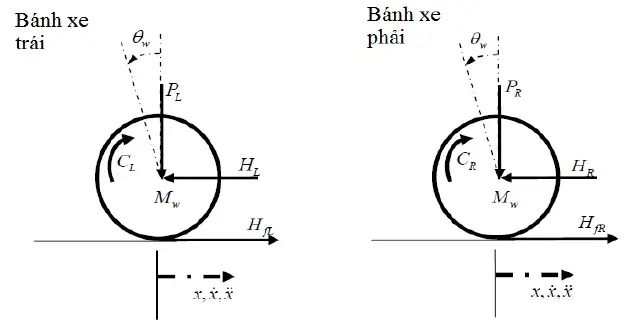
\includegraphics[width=1\textwidth]{pictures/wheel.png} 
            \caption{Sơ đồ tự do của các bánh}
        \end{figure}
        
        \hspace*{0.6cm}Áp dụng định luật 2 Newton cho phương ngang:
        \begin{align}
            \sum F_x &= M_w \ddot{x} = H_R - H_L 
        \end{align}
        
        Tổng moment quanh trọng tâm bánh xe:
        \begin{align}
            \sum M_o &= I_w \ddot{\theta} = C_R - H_R r 
        \end{align}
        
        Từ động học động cơ một chiều, moment quay động cơ được mô tả bởi:
        \begin{align}
            \tau_m = I_R \frac{d \omega}{dt} + \tau_a 
        \end{align}
        
        Với moment quay đầu ra:
        \begin{align}
            C = I_R \frac{d \omega}{dt} = -\frac{k_m k_e}{R} \dot{\theta}_w + \frac{k_m}{R} V_a 
        \end{align}
        
        Thay vào phương trình (1.2):
        \begin{align}
            I_w \ddot{\theta} = -\frac{k_m k_e}{R} \dot{\theta}_w + \frac{k_m}{R} V_a - H_R r 
        \end{align}
        
        Rút gọn biểu thức $H_R$:
        \begin{align}
            H_R = -\frac{k_m k_e}{Rr} \dot{\theta}_w  + \frac{k_m}{Rr} V_a - \frac{I_w}{r} \ddot{\theta}_w 
        \end{align}
        
        Phương trình (1.4) thay vào (1.1), ta thu được phương trình cho các bánh:
        
        \subsection*{Bánh xe bên trái}
            \begin{align}
                M_w \ddot{x} = -\frac{k_m k_e}{Rr} \dot{\theta}_w + \frac{k_m}{Rr} V_a - \frac{I_{w}}{r} \ddot{\theta}_w - H_L 
            \end{align}
        
        \subsection*{Bánh xe bên phải}
            \begin{align}
                M_w \ddot{x} = -\frac{k_m k_e}{Rr} \dot{\theta}_w  + \frac{k_m}{Rr} V_a - \frac{I_{w}}{r} \ddot{\theta}_w - H_R 
            \end{align}
        
        Bởi vì chuyển động tuyến tính được xem xét ở trọng tâm của bánh xe, góc quay có thể được biến đổi thành chuyển động tuyến tính bằng biến đổi đơn giản:
        \begin{align*}
            \ddot{\theta}_w r &= \ddot{x} \Rightarrow \ddot{\theta}_w = \frac{\ddot{x}}{r} \\
            \dot{\theta}_w r &= \dot{x} \Rightarrow \dot{\theta}_w = \frac{\dot{x}}{r}
        \end{align*}
       
        Bằng phép biến đổi tuyến tính, phương trình (1.7) và (1.8) có thể được viết lại như sau:
        \subsection*{Bánh xe bên trái}
        \begin{align}
            M_w \ddot{x} = -\frac{k_m k_e}{Rr^2} \dot{x} + \frac{k_m}{Rr^2} V_a - \frac{I_{w}}{r^2} \ddot{x} - H_L 
        \end{align}
        \subsection*{Bánh xe bên phải}
        \begin{align}
            M_w \ddot{x} = -\frac{k_m k_e}{Rr^2} \dot{x} + \frac{k_m}{Rr^2} V_a - \frac{I_{w}}{r^2} \ddot{x} - H_R 
        \end{align}
        \hspace*{0.6cm}Cộng 2 phương trình (1.9) và (1.10):
        \begin{align}
            2(M_w + \frac{I_w}{r^2})\ddot{x} = -\frac{2k_m k_e}{Rr^2} \dot{x} + \frac{2k_m}{Rr} V_a  - (H_L + H_R)
        \end{align}
    \section{Mô hình con lắc ngược}
        \hspace*{0.6cm}Cấu hình robot có thể được mô hình như một con lắc ngược
            \begin{figure}[H]
                \centering
                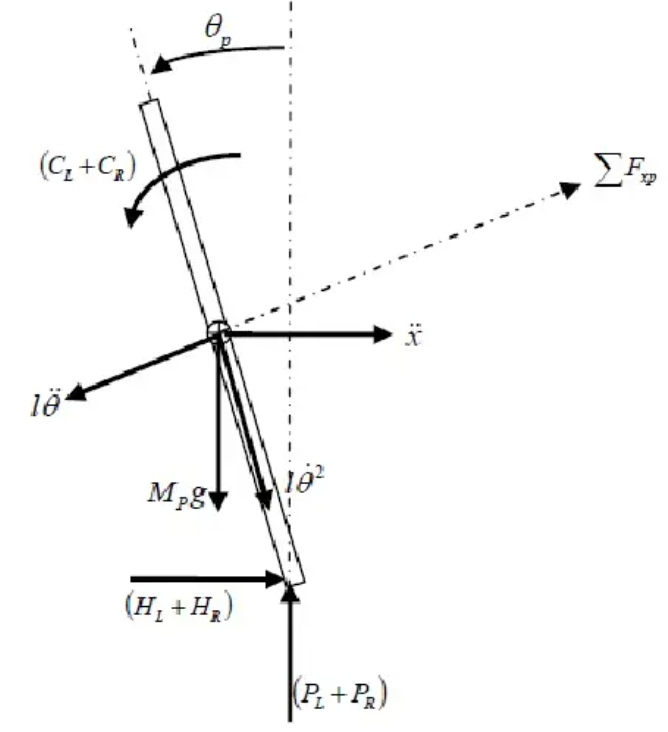
\includegraphics[width=0.5\textwidth]{pictures/inverted_pendulum.png} 
                \caption{Sơ đồ tự do của con lắc ngược}
            \end{figure}
        \subsection{Thiết lập hệ phương trình phi tuyến}
            Lặp lại, bằng việc sử dụng định luật 2 Newton, tổng các lực theo phương ngang:
            \begin{align}
                \sum F_x &= M_p \ddot{x} \nonumber\\
                (H_L + H_R) - M_p l \ddot{\theta} \cos &\theta_p + M_p l \dot{\theta}^2 \sin \theta_p = M_p \ddot{x} 
            \end{align}
            
            Suy ra:
            \begin{align}
                (H_L + H_R) &= M_p \ddot{x} + M_p l \ddot{\theta} \cos \theta_p - M_p l \dot{\theta}^2 \sin \theta_p 
            \end{align}
            
            Tổng các lực vuông góc với con lắc:
            \begin{align}
                \sum F_{xp} &= M_p \ddot{x} \cos \theta_p \nonumber\\
                (H_L + H_R) \cos \theta_p + (P_L + P_R) \sin& \theta_p - M_p g \sin \theta_p - M_p l \ddot{\theta}_p = M_p \ddot{x} \cos \theta_p 
            \end{align}
            
            Tổng moment quanh trọng tâm con lắc:
            \begin{align}
                \sum M_0 &= I_p a \nonumber \\
                -(H_L + H_R) l \cos \theta_p - (P_L + P_R) l&    \sin \theta_p - (C_L + C_R) = I_p \ddot{\theta} 
            \end{align}
            
            Moment quay áp dụng lên con lắc từ động cơ:
            \begin{align*}
                C_L + C_R = -\frac{2k_m k_e}{R} \frac{\dot{x}}{r} + \frac{2k_m}{R} V_a 
            \end{align*}
            
            Thay vào (1.15):
            \begin{align*}
                -(H_L + H_R) l \cos \theta_p - (P_L + P_R) l \sin \theta_p + \frac{2k_m k_e}{R} \frac{\dot{x}}{r} - \frac{2k_m}{R} V_a = I_p \ddot{\theta}_{p} 
            \end{align*}

            Do đó:
            \begin{align}
                -(H_L + H_R) l \cos \theta_p - (P_L + P_R) l \sin \theta_p = I_p \ddot{\theta}_{p} - \frac{2k_m k_e}{R} \frac{\dot{x}}{r} + \frac{2k_m}{R} V_a
            \end{align}

            Nhân phương trình (1.14) với $-l$ ta có:
            \begin{align*}
                -(H_L + H_R) l \cos \theta_p - (P_L + P_R) l \sin \theta_p + M_p g l \sin \theta_p + M_p l^2 \ddot{\theta}_p = -M_p l \ddot{x} \cos \theta_p 
            \end{align*}

            Thay thế phương trình (1.15) vào phương trình (1.16), ta được:

            \begin{equation}
                I_p \ddot{\theta}_p - \frac{2k_m k_e}{R} \frac{\dot{x}}{r} - \frac{2k_m}{R} V_a + M_p g l \sin\theta_p + M_p l^2 \ddot{\theta}_p = -M_p l \ddot{x} \cos\theta_p
            \end{equation}

            Để loại bỏ thành phần động học của động cơ \( (H_L + H_R) \), ta thay phương trình (1.13) vào phương trình (1.11), thu được:

            \begin{equation}
                2\left(M_w + \frac{I_w}{r^2} \right) \ddot{x} = -\frac{2k_m k_e}{R r^2} \dot{x} + \frac{2k_m}{R r} V_a - M_p \ddot{x} - M_p l \ddot{\theta}_p \cos\theta_p + M_p l \dot{\theta}_p^2 \sin\theta
            \end{equation}

            Kết hợp hai phương trình (1.17) và (1.18), ta có hệ phương trình chuyển động phi tuyến:

            \begin{align}
                (I_p +& M_p l^2)  \ddot{\theta}_p - \frac{2k_m k_e}{R r^2} \dot{x} + \frac{2k_m}{R r} V_a + M_p g l \sin\theta_p = -M_p l \ddot{x} \cos\theta_p  \\
                \frac{2k_m}{R r} V_a &= \left(2 M_w + \frac{2 I_w}{r^2} + M_p \right) \ddot{x} - \frac{2k_m k_e}{R r^2} \dot{x} + M_p l \ddot{\theta}_p \cos\theta_p - M_p l \dot{\theta}_p^2 \sin\theta_p 
            \end{align}

        \subsection{Tuyến tính hóa hệ phương trình}

            \hspace*{0.6cm}Để đơn giản và áp dụng điều khiển, ta giả sử:

            \[
            \theta_p = \pi + \phi
            \]

            Với \( \phi \) là một góc nhỏ so với phương thẳng đứng (tức là hệ đang dao động quanh vị trí thẳng đứng). Khi đó, các xấp xỉ tuyến tính:

            \[
            \cos\theta_p \approx -1, \quad \sin\theta_p \approx -\phi, \quad \left( \frac{d\theta_p}{dt} \right)^2 \approx 0
            \]

            Được áp dụng để đơn giản hóa hệ phương trình.

            Phương trình tuyến tính hóa của chuyển động là:

            \begin{equation}
                (I_p + M_p l^2)\ddot{\phi} - \frac{2k_m k_e}{R r} \dot{x} + \frac{2k_m}{R} V_a - M_p g l \sin \theta_p = M_p l \ddot{x}
            \end{equation}

            \begin{equation}
                \frac{2k_m}{R r} V_a = \left( 2M_w + \frac{2I_w}{r^2} + M_p \right) \ddot{x} + \frac{2k_m k_e}{R r^2} \dot{x} - M_p l \ddot{\phi}
            \end{equation}

            Để đưa hai phương trình trên về dạng phục vụ xây dựng mô hình không gian trạng thái, ta biến đổi:

            \begin{align}
                \ddot{\phi} &= \frac{M_p l}{(I_p + M_p l^2)} \ddot{x}
                + \frac{2k_m k_e}{R r (I_p + M_p l^2)} \dot{x}
                + \frac{2k_m}{R (I_p + M_p l^2)} V_a
                - \frac{M_p g l}{(I_p + M_p l^2)} \phi
                \\[1ex]
                \ddot{x} &= \frac{2k_m}{R r \left( 2M_w + \frac{2I_w}{r^2} + M_p \right)} V_a
                - \frac{2k_m k_e}{R r^2 \left( 2M_w + \frac{2I_w}{r^2} + M_p \right)} \dot{x}
                - \frac{M_p l}{\left( 2M_w + \frac{2I_w}{r^2} + M_p \right)} \ddot{\phi}
            \end{align}

            Nếu bỏ qua các thành phần quán tính kênh (ví dụ như động cơ), ta được:

            \begin{align}
                \ddot{\phi} + \frac{M_p g l}{I_p + M_p l^2} \phi &= \frac{2k_m}{R (I_p + M_p l^2)} V_a  \\[1ex]
                \ddot{x} + \frac{2k_m k_e}{(2M_w + \frac{2I_w}{r^2}) R^2} \dot{x} &= \frac{2k_m}{(2M_w + \frac{2I_w}{r^2}) R r} V_a
            \end{align}

            \noindent
            \hspace*{0.6cm}Trong mô hình này, giả thiết rằng bánh xe luôn tiếp xúc với mặt đất và không có trượt. Các lực quay và ma sát được bỏ qua.

            \subsection{Mô hình không gian trạng thái}

            \hspace*{0.6cm}Từ các phương trình đã tuyến tính hoá, ta xây dựng hệ phương trình không gian trạng thái dưới dạng:

            \begin{equation}
                \begin{bmatrix}
                    \dot{\phi} \\
                    \ddot{\phi}
                \end{bmatrix}
                =
                \begin{bmatrix}
                    0 & 1 \\
                    -\dfrac{M_p g l}{I_p + M_p l^2} & 0
                \end{bmatrix}
                \begin{bmatrix}
                    \phi \\
                    \dot{\phi}
                \end{bmatrix}
                +
                \begin{bmatrix}
                    0 \\
                    \dfrac{2k_m}{(I_p + M_p l^2) R}
                \end{bmatrix}
                 V_a
            \end{equation}

            \begin{equation}
                \begin{bmatrix}
                    \dot{x} \\
                    \ddot{x}
                \end{bmatrix}
                =
                \begin{bmatrix}
                    0 & 1 \\
                    0 & -\dfrac{2k_m k_e}{(2M_w + \frac{2I_w}{r^2}) R^2}
                \end{bmatrix}
                \begin{bmatrix}
                    x \\
                    \dot{x}
                \end{bmatrix}
                +
                \begin{bmatrix}
                    0 \\
                    \dfrac{2k_m}{(2M_w + \frac{2I_w}{r^2}) R r}
                \end{bmatrix}
                V_a
            \end{equation}
    \section{Hàm truyền hệ thống}
        \hspace*{0.6cm}Trong phạm vi nghiên cứu này, ta chỉ tập trung vào phương trình liên quan đến góc nghiêng $\phi$, vì đây là yếu tố quyết định đến khả năng giữ thăng bằng của robot. Việc duy trì $\phi$ gần bằng 0 giúp hệ thống đứng vững, trong khi sai lệch lớn sẽ dẫn đến mất cân bằng.

        Do đó, để đơn giản hoá mô hình và tập trung vào mục tiêu ổn định hoá con lắc ngược, ta sử dụng phương trình (1.27) và không xét đến phương trình vị trí $x$ trong các phân tích và thiết kế điều khiển tiếp theo.

        Phương trình vi phân bậc hai của hệ được viết lại như sau:
        
        \begin{equation}
            \ddot{\phi} + \frac{M_p g l}{I_p + M_p l^2} \phi = \frac{2k_m}{R (I_p + M_p l^2)} V_a
        \end{equation}
        
        Gọi:
        
        \[
            x_1(t) = \phi(t), \quad x_2(t) = \dot{\phi}(t)
        \]
        
        Khi đó hệ phương trình trở thành:
        
        \[
        \begin{cases}
            \dot{x}_1(t) = x_2(t) \\
            \dot{x}_2(t) = -\frac{M_p g l}{I_p + M_p l^2} x_1(t) + \frac{2k_m}{R (I_p + M_p l^2)} V_a
        \end{cases}
        \]
        
        Biểu diễn dưới dạng ma trận không gian trạng thái:
        
        \begin{equation}
        \begin{bmatrix}
            \dot{x}_1(t) \\
            \dot{x}_2(t)
        \end{bmatrix}
        =
        \begin{bmatrix}
            0 & 1 \\
            -\frac{M_p g l}{I_p + M_p l^2} & 0
        \end{bmatrix}
        \begin{bmatrix}
            x_1(t) \\
            x_2(t)
        \end{bmatrix}
        +
        \begin{bmatrix}
            0 \\
            \frac{2k_m}{R (I_p + M_p l^2)}
        \end{bmatrix}
        V_a
        \end{equation}
        
        Với đầu ra \( y(t) = \phi(t) = x_1(t) \Rightarrow \)
        
        \[
        y(t) = \begin{bmatrix} 1 & 0 \end{bmatrix}
        \begin{bmatrix}
            x_1(t) \\
            x_2(t)
        \end{bmatrix}
        \]
        
        \textbf{Giá trị các thông số:}
        \[
            M_p = 1.2 \, \text{kg}, \quad g = 9.81, \quad l = 0.1, \quad I_p = 0.01, \quad k_m = 0.28, \quad R = 5.25 \, \Omega
        \]
        
        Thay số vào ta có ma trận hệ:
        
        \[
            A = \begin{bmatrix} 0 & 1 \\ -53.51 & 0 \end{bmatrix}, \quad
            B = \begin{bmatrix} 0 \\ 4.85 \end{bmatrix}, \quad
            C = \begin{bmatrix} 1 & 0 \end{bmatrix}, \quad
            D = 0
        \]
        
        Từ mô hình không gian trạng thái, ta có:
        
        \[
        G(s) = C(sI - A)^{-1}B
        \]
        
        Tính:
        
        \[
        sI - A =
        \begin{bmatrix}
            s & -1 \\
            -53.51 & s
        \end{bmatrix}, \quad
            (sI - A)^{-1} = \frac{1}{s^2 + 3.51}
        \begin{bmatrix}
            s & 1 \\
            -53.51 & s
        \end{bmatrix}
        \]
        
        Do đó:
        
        \begin{align*}
            G(s) &= \begin{bmatrix} 1 & 0 \end{bmatrix}
            \cdot \frac{1}{s^2 + 53.51}
        \begin{bmatrix}
            s & 1 \\
            -53.51 & s
        \end{bmatrix}
        \cdot
        \begin{bmatrix}
            0 \\
            4.85
        \end{bmatrix} \\
        &= \frac{1}{s^2 + 3.51} \cdot \begin{bmatrix} 1 & 0 \end{bmatrix}
        \cdot
        \begin{bmatrix}
            4.85
        \end{bmatrix}
        = \frac{1.85}{s^2 + 53.51}
        \end{align*}
        
        \textbf{Vậy:}
        \[
            G(s) = \frac{4.85}{s^2 + 53.51}
        \]
        
        Đây là hàm truyền từ điện áp điều khiển \( V_a \) đến góc lệch \( \phi(t) \) của con lắc ngược.
    \section{Kết luận}
        \hspace*{0.6cm}Sau khi thực hiện quá trình mô hình hóa, tuyến tính hóa và xây dựng hệ phương trình không gian trạng thái, ta đã thu được hàm truyền tuyến tính biểu diễn mối quan hệ giữa điện áp điều khiển đầu vào $V_a$ và góc nghiêng $\phi$ của robot hai bánh:

        \[
        G(s) = \frac{4.85}{s^2 + 53.51}
        \]
        
        Hàm truyền trên cho thấy hệ thống là một hệ dao động bậc hai không có thành phần tắt dần (damping) và có tính chất **marginally stable** (ổn định biên). Điều này là đặc trưng của mô hình con lắc ngược: hệ không ổn định khi không có điều khiển tác động.
        
        Việc xây dựng được hàm truyền là một bước quan trọng, tạo nền tảng để thiết kế các bộ điều khiển như PID, LQR hoặc các chiến lược điều khiển hiện đại nhằm đảm bảo robot giữ được trạng thái cân bằng và theo dõi quỹ đạo mong muốn.
        
        Trong chương tiếp theo, ta sẽ tiến hành thiết kế và mô phỏng các bộ điều khiển dựa trên hàm truyền đã thu được.
            
        
       